\section{Alimentation}
Nous avons vu que la remorque utilise une prise 13 broches pour son alimentation. Le véhicule tractant la remorque peut varier, il n'y a donc pas de
garanti qu'il y ait une deuxième prise disponibles pour le système qui sera ajouté. L'idéal serait d'avoir accès à la masse et au 12[V].
\begin{figure}[H]
    \centering
    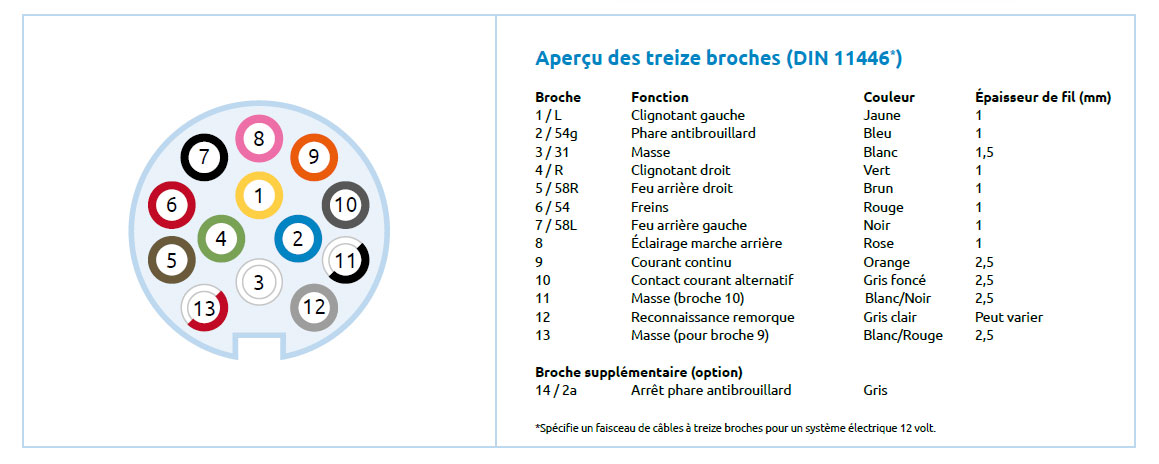
\includegraphics[width=14cm]{assets/figures/broches.jpg}
    \caption{Sortie prises 13 broches - \cite{prise}}
\end{figure}
Ce qui nous intéresse:
\begin{itemize}
    \item Broche 9  : 12 [V]
    \item Broche 13 : Masse
\end{itemize}
Les broches ayant chacunes une fonction particulière, il n'existe pas de multiprise permettant de joindre deux connecteurs mâle vers une femelle.
Il faudrait donc fabriquer un boitier d'adaptation permettant de dévier les broches utiles, tout en préservant l'alimentation de la remorque et du matériel installé dessus.


Voir figure \ref{alim}.
\begin{figure}[h]
    \centering
    \includegraphics[width=7cm]{assets/figures/Alimentation.drawio}
    \caption{Boitier d'adaptation de l'alimentation \label{alim}}
\end{figure}
\newpage

\section{Communication}
Dans le cadre de ce projet, plusieurs éléments devront communiquer entre eux, notamment l'unité de traitement d'image,
l'actionnement de la télécommande ainsi que le retour vidéo pour le copilote, il est donc important de définir comment ils communiqueront entre eux.
Il est important de se rappeler que leurs emplacements seront les suivants:

\begin{table}[h]
    \begin{center}
        \caption{Liste des élements et emplacements}
        \begin{tabular}{|c|l|}
            Elements                        & Emplacement                \\ \hline
            Caméra et boitier de traitement & Support de la remorque     \\
            Eclairage                       & Timon                      \\
            Actionnement de la télécommande & Support de la remorque     \\
            Affichage pour copilote         & Place passager du véhicule
        \end{tabular}
    \end{center}
\end{table}

Dans notre cas de figure, les élements sont concentrés sur la remorque et dans le véhicule tractant. La communication cablée est possible
entre la caméra, le boitier, l'actionnement de la télécommande et éventuellement l'éclairage si celui-ci à besoin d'être contrôlé spécifiquement.
En ce qui concerne le retour vidéo, il se trouvera principalement dans l'habitacle du véhicule, mais pourrait également être emporté autour du véhicule,
dans ce cas, la connexion filaire n'est pas envisageable.

Parmis les connexions sans fil:
\begin{itemize}
    \item Via une connexion Bluetooth.
    \item Via un réseau \Gls{wifi} local.
\end{itemize}
La connexion sans fil doit garantir une connectivité stable sur un rayon de 5 mètres autour du véhicule (avec obstacles). De plus, le débit doit être
suffisant pour diffuser un flux vidéo (entre 30 et 60 \Gls{fps}). La solution du réseau local \Gls{wifi} semble être la meilleure.

\textbf{La possibilité de communiquer via un réseau local \Gls{wifi} devient donc un prérequis pour le retour vidéo.}
\newpage
\section{Capture et traitement d'image}
\subsection{Eclairage}
La sélection de l'éclairage va dépendre des points suivants:
\begin{itemize}
    \item La longueur d'onde nécessaire.
    \item L'emplacement de l'éclairage
    \item La taille du champ à éclairer.
\end{itemize}
Le premier point s'est défini durant la phase de recherche, l'idéal serait d'avoir une source émettant une onde de 850 \si{\nano\metre}.

Les deux points suivants sont liés, l'éclairage sera monté sur le timon et le but est d'éclairer le sol sur une largeur d'environ 160 \si{\centi\metre} (correspondant aux champ d'actions du semoir),
c'est à dire sur une bande. Avec des leds montées en ligne, il n'est pas nécessaire qu'elles aient un grand angle de diffusion.

Des leds trouvées sur le site de Mouser semblent correspondre à ces conditions \cite{ledIR}.

Leur préparation se résumerait à une mise en bande (2x 80\si{\centi\metre}) et les alimenter.


\subsection{Caméra}
La caméra à choisir doit remplir les critères suivants:
\begin{itemize}
    \item Pas de filtre IR (ou facilement retirable).
    \item Compatible avec une carte de traitement d'image.
    \item Champ de vision suffisant pour observer la largeur de la route.
\end{itemize}

La caméra Module 3 "NoIR - Wide" de Rapsberry Pi \cite{camera} semble répondre aux critères. Avec une mise au point à partir de 5cm vers l'infini,
une résolution de 11.9 mégapixels (4608x2592) et d'un champ de vision de \ang{120}, elle offre une image nette et très détaillée avec beaucoup de liberté sur
son placement. Sa sensibilité aux infrarouges monte jusqu'au environ de 1000 \si{\nano\metre}.
\begin{figure}[H]
    \centering
    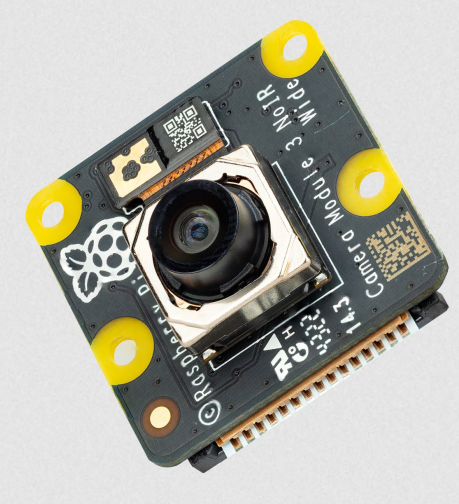
\includegraphics[height=7cm,angle=-90]{assets/figures/camera.png}
    \caption{Camera module 3 NoIR wide}
\end{figure}

\subsection{Système embarqué de traitement}
\begin{itemize}
    \item Peu encombrant.
    \item Relativement puissant.
    \item Communication WiFi en tant qu'émetteur.
    \item Compatible avec la caméra.
\end{itemize}
Rapsberry Pi 4.


\section{Système de commande}
\subsection{Actionneurs de la télécommande}
Les idées de base d'actionneurs permettant d'appuyer sur la télécommande sont les suivants:
\begin{listage}
    1. Vérins électriques.\\
    2. Servomoteurs.\\
    3. Moteurs pas à pas.
\end{listage}

Les vérins électriques ont l'avantages d'être facile à installer, il suffirait d'une plaque de support perforée au dessus de chaque bouton et d'y insérer
les pièces à la profondeur souhaitée, puis de les actionner/rétracter pour appuyer ou non sur un bouton. Cependant, les vérins disponibles sur le marché semblent être surdimensionnés pour la tâche en question, les forces et
consommation pour un fonctionnement normal sont très grand. Les prix sont également très élevé, il est difficile de trouver des pièces de moins de 100 CHF l'unité
pour les dimensions désirées. De plus, les délais de livraison durant la période dédiée au développement de se projet sont relativements incertains pour se genre de pièce.

L'idée, avec les servomoteurs, serait de les équiper d'un élement de préhension tangent à l'axe de rotation du moteur permettant de presser sur les boutons.
Le pilotage d'un servomoteur se fait par PWM, nécessitant donc qu'une seule sortie par élements au niveau de la carte de commande. De plus, il est assez facile de
trouver des servomoteurs avec des caractéristiques en phase avec le projet, c'est à dire d'un point de vu taille, force et consommation, et ce à des prix
raisonnable (avoisinant les 5 à 10 CHF). L'installation sur un support est plus complexe que pour les vérins.

L'utilisation du moteur pas à pas serait similaires au servomoteur, c'est à dire avec un élement qui presse sur les boutons.
Il est assez facile de trouver des moteurs avec des caractéristiques en phase avec le projet à des prix résonnable (avoisinnant 10 CHF). La commande d'un moteur pas à pas
se fait usuellement via un pilote servant d'interface entre le moteur et la carte de commande. Il est nécessaire d'avoir une carte pilote par moteur (environ 10 CHF par unité).
L'installation sur un support est plus complexe que pour les vérins.

Avec ces informations, en comparant prix, facilité d'acquisition, pilotage, caractéristique obtenable, délai de livraison, la solution du servomoteur semble être la plus
appropriée.\textbf{Je vais donc baser la suite du développement avec des servomoteurs comme actionneurs de la télécommande.}

\subsection{Pilotage des actionneurs}
La carte de commande servant à piloter les servomoteurs devra être capable de:
\begin{listage}
    1. Commander 6 servomoteurs simultanément.\\
    2. Communiquer (reçevoir des informations) avec le boitier de traitement d'image.\\
    3. Afficher un statut via un voyant (une led par exemple).
\end{listage}

Plusieurs possibilités se présentent , parmis la famille des Arduinos:
\begin{table}[H]
    \begin{center}
        \caption{Liste de cartes embarqueés}
        \begin{tabular}{|l|l|l|l|}
            Cartes                & Sortie PWM & Prix moyen   & Module \Gls{wifi} intégré? \\ \hline
            Arduino Nano          & 6          & 20 \Gls{chf} & Non                        \\
            Arduino Micro         & 7          & 25 \Gls{chf} & Non                        \\
            Arduino Uno           & 6          & 30 \Gls{chf} & Non                        \\
            Arduino Mega          & 15         & 40 \Gls{chf} & Non                        \\
            Arduino MKR WiFi 1010 & 10         & 35 \Gls{chf} & Oui
        \end{tabular}
    \end{center}
\end{table}\\

Les 4 premières cartes présentent cochent 2 parmis les 3 prérequis de sélection. Ce qui les différentie c'est majoritairement le coût, l'encombrement et la vitesse de travail.
Au vu de la simplicité des tâches, un Nano ou Micro serait suffisant. En imaginant que la communication avec l'unité de traitement d'image se fasse via un réseau \Gls{wifi} local,
il faudrait ajouter un module spécifique permettant la connexion, par exemple l'ESP8266.\\
En plus de pouvoir commander les servomoteurs et d'afficher un statut, le MKR WiFi 1010 possède un module \Gls{wifi} préintégré.
Les prix entre les cartes avec l'ajout d'un module et le MKR WiFi 1010 sont plus ou moins semblable. Ce dernier offre l'avantage d'être compacte et de limiter le câblage.
\textbf{Je vais donc baser la suite du développement avec l'Arduino MKR WiFi 1010.} \cite{MKR}
\section{Retour vidéo}
Le résultat de l'analyse du traitement d'image et la mise en évidence des traces d'hydrocarbure doivent être visible par le copilote.
La visualisation du retour se fera naturellement via un écran. Les idées de bases sont les suivantes:
\begin{itemize}
    \item Installation d'un écran portable.
    \item Affichage via une application mobile.
    \item Affichage via une page web locale.
\end{itemize}

Les problèmes de l'écran portable sont multiples, notamment l'alimentation, le câblage vers une source d'alimentation peut-être encombrant
et limiterait les mouvements/déplacements de l'utilisateur. De plus la connexion vers un réseau \Gls{wifi} local n'est pas garantie.

L'idée de l'application mobile présente certains avantages, comme l'installation unique. L'opérateur n'aurait qu'à mettre l'application
qu'une seul fois sur son téléphone portable pour accéder au retour vidéo (sous condition d'être connecté au réseau \Gls{wifi} local).
Tout le monde serait alors équiper de son propre écran, petit, pratique et peu encombrant. Le problème majeur est la différence de système d'exploitation
entre les téléphones portables. Le développement d'une application universelle est compliquée, il faudrait avoir une application par système grand public.
De plus, l'installation d'une application non reconnu par Apple doit être téléversée directement à partir d'un ordinateur.

L'affichage du retour vidéo via une page locale semble être optimal. En plus de regrouper les avantages de l'application mobile, nous nous débarrassons des défauts.
L'accès au lien de la page pourrait se faire via un QR code à scanner sur le boitier de commande.

\textbf{L'affichage se fera via une page web locale.}

\section{Résumé des décisions}
\begin{table}[H]
    \begin{center}
        \caption{Table de résumé des décisions}
        \begin{tabular}{|c|l|}
            Elements                  & Solutions                         \\ \hline
            Communication             & Filaire + Réseau \Gls{wifi} Local \\
            Caméra                    & Rpi module 3 NoIR Wide            \\
            Traitement d'image        & Rapsberry Pi 4                    \\
            Actionnement télécommande & Servomoteurs                      \\
            Commande actionneurs      & Arduino MKR WiFi 1010 \cite{MKR}  \\
            Affichage pour copilote   & Page web local                    \\
        \end{tabular}
    \end{center}
\end{table}

